%! TeX program = pdflatex
\documentclass{article}
\usepackage[english]{babel}
\usepackage[utf8]{inputenc}
\usepackage{amsmath}
\usepackage{amssymb}
\usepackage{minted}
\usepackage{listings}
\usepackage{xcolor}
\usepackage{graphicx}
\usepackage{pgf}
\usepackage{algorithm}% http://ctan.org/pkg/algorithms
\usepackage{algorithmicx}
\usepackage{algpseudocode}% http://ctan.org/pkg/algorithmicx
% \usepackage{tikz-cd}
\usepackage{listings}
\usepackage{xcolor}
\usepackage{tikz}
\usepackage{comment}
\usepackage{float}
\usepackage{circuitikz}
% \usetikzlibrary{shapes, arrows, positioning}
% \lstset{ 
%     language=Python,                 % the language of the code
%     basicstyle=\ttfamily\small,      % the size of the fonts that are used for the code
%     numbers=left,                    % where to put the line-numbers
%     numberstyle=\tiny\color{gray},   % the style that is used for the line-numbers
%     stepnumber=1,                    % the step between two line-numbers. If it's 1, each line will be numbered
%     numbersep=5pt,                   % how far the line-numbers are from the code
%     backgroundcolor=\color{white},   % choose the background color. You must add \usepackage{color}
%     showspaces=false,                % show spaces adding particular underscores
%     showstringspaces=false,          % underline spaces within strings
%     showtabs=false,                  % show tabs within strings adding particular underscores
%     frame=single,                    % adds a frame around the code
%     rulecolor=\color{black},         % if not rolframe-color may be changed on line-breaks within not black text (e.g. comments (green here))
%     tabsize=4,                       % sets default tabsize to 4 spaces
%     captionpos=b,                    % sets the caption-position to bottom
%     breaklines=true,                 % sets automatic line breaking
%     breakatwhitespace=false,         % sets if automatic breaks should only happen at whitespace
%     title=\lstname,                  % show the filename of files included with \lstinputlisting; also try caption instead of title
%     keywordstyle=\color{blue},       % keyword style
%     commentstyle=\color{green},      % comment style
%     stringstyle=\color{red},         % string literal style
%     escapeinside={\%*}{*)},          % if you want to add LaTeX within your code
%     morekeywords={*,...} 
% }            % if you want to add more keywords to the rol\newenvironment{notation}
\newtheorem{remark}{Remark}
\newtheorem{definition}{Definition}
\newtheorem{property}{Property}

\setlength\parindent{0pt}

\newcommand{\pder}[2]{\frac{\partial #1}{\partial #2}}

\title{Decentralized Grid Control in COLMENA \\ Activity 3}
\author{Pablo de Juan Vela $^{1}$, Marco Muttoni $^{1}$, Josep Fanals i Batllori $^{1}$ \\
        \small $^{1}$eRoots Analytics, Barcelona, Spain \\
}
\date{\today}

\usepackage[style=ieee]{biblatex}
\addbibresource{ref.bib}
\setlength{\parskip}{1em} 
\begin{document}
\maketitle
\section{Introduction}
COLMENA aims to enable decentralized decision-making by coordinating autonomous agents that perform specific roles. Each agent can execute certain roles to impact the system and operate based on local measurements and predictions. This project uses COLMENA to deploy a multi agent control system in where each agent is responsible for the control of a specific area. The different agents use the tools available through COLMENA to ensure proper coordination for completing the goal of controlling the frequency throughout the grid.

Distributed Model Predictive Control (MPC) is a particularly well-suited control strategy in this context. MPC anticipates future states and disturbances, optimizes control actions over a prediction horizon, and incorporates constraints in a clear manner. When implemented in a distributed fashion through COLMENA, each agent can locally solve an MPC problem to manage its area, while coordinating with neighboring agents to respect power flow constraints and system-wide objectives.

This report will first explain the physical models and equations used to build the MPC, we will then explain the optimisation background used for to implement the Distributed MPC, and finally we will use the MPC control in the IEEE 39-bus grid, as found in \cite{grids:ieee39}, through ANDES to showcase its capability for frequency control.

\newpage
\section{Modeling}
Accurate modeling of the contingencies that are likely to take place in the grid, as well as the frequency and angle dynamics of each area, are fundamental to the design and implementation of distributed control strategies in power systems. It is central to capture how each area responds to generation-demand imbalances and how it interacts electrically with neighboring regions through phase angle differences whenever a contingency takes place. By understanding these behaviors, the proposed MPC can anticipate future states and choose the appropriate controls actions.

\subsection{Contingency definition}
In power systems, contingencies refer to unexpected events or disturbances that can significantly impact the system's stability and operation. These events can range from equipment failures to sudden changes in load or generation, and they require immediate response from control systems to maintain grid stability and prevent cascading failures \cite{contingency:analysis}. Not surprisingly, the recent Spanish blackout that took place last April was a clear example of such cascading events. Contingencies can be caused by multiple, being the most common types of contingencies the following:

\begin{itemize}

\item \textbf{Generation contingencies:} these involve the sudden loss of generating units due to mechanical failures, protection system trips, or fuel supply issues. Generator outages can cause immediate power imbalances, leading to frequency deviations and potential voltage problems. The severity depends on the size of the lost generation relative to the system's total capacity and available reserves. Most often, loss of generation causes the frequency to drop, which has to be counteracted by the control actions of other generation units, or also the reduction or even disconnection of loads \cite{marzband2016adaptive}. 

\item \textbf{Transmission line contingencies:} these occur when transmission lines are disconnected due to faults, protection system operation, or physical damage (also linked weather events or equipment failure). Line outages can cause power flow redistributions, potentially leading to overloaded remaining lines and voltage violations, which can further exacerbate the frequency deviations and result in a complete blackout of the system. Restorative actions can involve the quick re-connection of the line, the re-routing of the power flow by adjusting the setpoints of nearby elements, or running an optimal transmission switching algorithm to find the best positions of the switches and disconnectors. However, a strong power grid must also be properly planned and dedicate a budget for transmission expansion planning \cite{aeggegn2020load}. 

\item \textbf{Load contingencies:} sudden changes in load demand, such as the disconnection of large industrial loads or the connection of significant new loads, can create power imbalances. While load increases typically cause frequency drops, load decreases can cause frequency rises \cite{contingency:load}. On the other hand, loads are also employed to provide flexibility to the system, by adjusting the associated consumption to meet the requirements imposed by the transmission system operator, which are eventually monetarily compensated. Even though loads are constantly changing in the system, we define load contingencies as sudden and large spikes in demand, akin to the connection or disconnection of massive consumption points.

\item \textbf{Weather-related contingencies:} extreme weather events such as storms, lightning strikes, or high winds can cause multiple simultaneous contingencies, including line outages, equipment damage, and load changes. These events often require coordinated responses across multiple control areas \cite{contingency:weather}. It is often the case that a weather-related event can simultaneously cause a generation contingency and a transmission line contingency. Hence, power grids are sometimes designed to meet not only the N-1 criterion, but also the N-2 criterion, which is the ability to withstand two contingencies at the same time.

\item \textbf{Equipment failures (others):} other contingencies can be due to failures in critical equipment such as transformers, circuit breakers, or protection systems that can further lead to cascading effects throughout the system. These failures can be caused by aging, improper maintenance, or external factors \cite{li2006power}. In practical terms, and when seen from a modelling perspective, these equipment failures are not different from the aforementioned contingency types, as they can cause a sudden frequency variation and also a power flow redistribution. 

\end{itemize}

The impact of contingencies on power system dynamics can be characterized by their severity, duration, and propagation characteristics. Severe contingencies can lead to frequency excursions that exceed normal operating limits, potentially triggering automatic load shedding or generator tripping to prevent system collapse \cite{contingency:stability}.

In the context of distributed control systems like COLMENA, contingencies create the need for coordinated responses across multiple areas. The distributed MPC framework must be able to detect the impact of these events in the electrical magnitudes under measurement, assess their influence on local and neighboring areas, and coordinate appropriate control actions to restore system stability while respecting operational constraints. Figure \ref{fig:contingencies} shows a schematic representation of the contingencies under study.

\begin{figure}[ht]
    \centering
    \begin{circuitikz}[scale=1.2]
        % Define coordinates
        \coordinate (A) at (0,0);
        \coordinate (B) at (4,0);
        \coordinate (C) at (8,0);
        \coordinate (D) at (4,2);
        \coordinate (E) at (4,-2);
        
        % Area 1 - Left side
        \draw[thick, blue] (-1,1) rectangle (3,-1);
        \node[blue] at (1,1.6) {\textbf{Area 1}};
        
        % Area 2 - Right side  
        \draw[thick, red] (5,1) rectangle (9,-1);
        \node[red] at (7,1.6) {\textbf{Area 2}};
        
        % Generators
        \node[above] at (1,0.25) {$G_1$};
        \node[above] at (7,0.25) {$G_2$};
        
        % Loads
        \node at (1,-0.5) {$L_1$};
        \node at (7,-0.5) {$L_2$};
        
        % Transmission line
        \draw[thick] (3,0.5) -- (5,0.5);
        % \draw[thick] (4,1) -- (4,0.5);
        
        % Line label
        \node[above] at (4,0.5) {$L_{12}$};
        
        % Contingency scenarios
        % 1. Generator disconnection (G1)
        \draw[red, thick, dashed] (1,0.5) circle (0.4);
        \node[red, above] at (1,-0.29) {\textbf{Gen. Outage}};
        
        % 2. Load disconnection (L2)
        \draw[orange, thick, dashed] (7,-0.5) circle (0.4);
        \node[orange, above] at (7,-0.18) {\textbf{Load Increase}};
        
        % 3. Line opening (L12)
        \draw[purple, thick, dashed] (4.0,0.7) circle (0.4);
        \node[purple, above] at (4,1.2) {\textbf{Line Outage}};
        
        % Frequency indicators
        \node[blue] at (1,1.2) {$f_1(t)$};
        \node[red] at (7,1.2) {$f_2(t)$};
        
        % Power flow arrows
        \draw[->, thick, blue] (2.5,0.5) -- (2.8,0.5);
        \draw[->, thick, red] (5.2,0.5) -- (5.5,0.5);
        
        % Legend
        \node[align=left] at (4,3.0) {
            \textbf{Contingency Types:} \\
            \textcolor{red}{\textbf{---}} Generation Outage \\
            \textcolor{orange}{\textbf{---}} Load Shedding \\
            \textcolor{purple}{\textbf{---}} Line Opening
        };
        
    \end{circuitikz}
    \caption{Schematic representation of the power system contingencies under analysis showing generation outage, load shedding, and line opening events in a two-area system.}
    \label{fig:contingencies}
\end{figure}


\subsection{Connection/disconnection definition}
In modern power systems, it is increasingly common to integrate new entities, such as solar parks or other renewable energy sources. The connection of a new component means that both the new entity and the rest of the system must detect the change and adapt, ensuring that the added installation does not negatively impact, and ideally improves, the operation of the electrical grid.

From a modeling and control perspective, the connection or disconnection of system elements, whether they are generators, loads, or other devices, can be treated as a particular case of contingency. The system must respond to these events in much the same way as it does to faults or sudden disturbances: by rebalancing power flows, adjusting control actions, and maintaining stability.

For this reason, in our framework, the connection or disconnection of components is not fundamentally different from other contingencies. Both require the system to adapt dynamically, leveraging distributed control and coordination among agents to ensure continued secure and efficient operation.

To test the system's adaptability, we consider scenarios involving the connection and disconnection of power injection sources, both generators and loads, to observe how the agents adjust their behavior. In both cases, the distributed control architecture must detect the change, coordinate the necessary adjustments, and maintain the desired performance of the grid.

\subsection{Grid dynamics}
In the proposed framework, each electrical area is represented using two states values:
\begin{itemize}
    \item \textbf{Frequency} $f_i(t)$: the local frequency of area $i$, which reflects the balance between generation and consumption.
    \item \textbf{Phase Angle} $\delta_i(t)$: the relative voltage phase angle of area $i$ with respect to the reference area, governing power exchanges with neighboring areas.
\end{itemize}
This abstraction treats each area as a coherent group of generators and loads that tend to oscillate together in response to disturbances. It enables scalable distributed control by reducing the system's dimensionality.

The frequency evolution in each area is governed by a version of the swing equation:
\begin{equation}
    M_i \frac{df_i(t)}{dt} = -D_i(f_i(t) - f_0) + \sum_{k \in \text{Area}_i} P^{\text{gen}_k}_{t} - \sum_{j \in \mathcal{N}_i} P^{i,j}_t - P^{\text{demand}}_i(t)
\end{equation}
where:
\begin{itemize}
    \item $M_i$ is the aggregated inertia of area $i$,
    \item $D_i$ is the damping coefficient of area $i$,
    \item $f_0$ is the nominal frequency (e.g., 50 or 60 Hz),
    \item $P^{\text{gen}_k}_t$ is the generation in area $i$,
    \item $P^{i,j}_t$ is the power exchanged from $i$ to area $j$.
\end{itemize}

The relative angle $\delta_i(t)$ accumulates the frequency deviation with the reference area over time:
\begin{equation}
    \frac{d\delta_i(t)}{dt} = 2\pi(f_i(t) - f_0)
\end{equation}
This relation ensures that the angle reflects the integral of frequency deviation, which is crucial for tracking system phase shifts over time. 


In this formulation, we use the DC power flow approximation to model the active power exchange between areas. This approach is widely accepted in high-voltage transmission system analysis due to its simplicity and relatively high accuracy under typical operating conditions. The approximation is based on the following assumptions:
\begin{itemize}
    \item Voltage magnitudes are close to their nominal values and are considered constant.
    \item Angle differences between buses are small enough that $\sin(\delta_i - \delta_j) \approx \delta_i - \delta_j$.
    \item Line resistance is negligible compared to reactance, so power losses are ignored.
\end{itemize}
Under these assumptions, the active power flow from area $i$ to area $j$ can be approximated by, this shows that active power flows are driven by angle differences and line susceptance $B_{i,j}$.:
\begin{equation}
    P^{i,j}_t = B_{i,j}(\delta_i(t) - \delta_j(t))
\end{equation}
where $B_{i,j}$ represents the total susceptance between the two areas. This is calculated as the sum of the susceptances of all transmission lines directly connecting buses in area $i$ to buses in area $j$:
\begin{equation}
    B_{i,j} = \sum_{\text{line i connects area i to area j}} b_{\text{line i}}
\end{equation}
This aggregation allows us to ignore the specific topologies of the areas during inter-area coordination, while still capturing the essential physics of power exchange via angle differences. It also reduces computational complexity, which is critical for scalable distributed optimisation.

\subsection{Grid Controls}
We build a multi-agent system where each agent is responsible for the control of a defined electrical area. Each area comprises several buses, generators, and loads, and interacts with other areas through lines. The objective of the agent is to maintain frequency stability by coordinating with neighboring agents through the sharing of information. 

Each agent is equipped with the capability to perform multiple control functions within its domain, depending on the system design and available actuators. These actions may include:
\begin{itemize}
    \item \textbf{Power generation control}: adjusting generator outputs to balance load and maintain frequency.
    \item \textbf{Load shedding strategies}: curtailing controllable loads during contingencies to stabilize frequency.
    \item \textbf{Battery or storage management}: charging or discharging storage systems to buffer fluctuations in net demand or generation.
    \item \textbf{Reactive power or voltage support}: engaging voltage control mechanisms to assist in voltage regulation, if needed.
\end{itemize}

In the broader COLMENA framework, agents could also be capable of activating other roles local roles, provided that the dynamics and interactions of those roles are explicitly defined and known by the agent.

In this first implementation, we focus on a simplified setting where each agent directly controls the ramp of generator power outputs within its area. Specifically, the control vector \( u_i \) for agent \( i \) is defined as the difference in power output between two consecutive time steps:
\begin{equation}
    u_i(t) = P^{\text{gen}}_i(t+1) - P^{\text{gen}}_i(t) \in \mathbb{R}^{n_{g,i}}
\end{equation}
where \( P^{\text{gen}}_i(t) \) is the vector of generator power outputs at time \( t \), and \( n_{g,i} \) is the number of controllable generators in area \( i \).

The control inputs are subject to ramp-rate constraints that limit how fast the generators can increase or decrease their output:
\begin{equation}
    u^{\min}_{k} \leq u_{i,k}(t)  \Delta  t \leq u^{\max}_{k} \quad \forall k \in \{1, \dots, n_{g,i}\}, \forall t
\end{equation}
where \( u^{\min}_{k} \) and \( u^{\max}_{k} \) are the ramp-down and ramp-up limits (in pu/s) for generator \( k \). 

\newpage
\section{Mathematical Formulation}
A Model Predictive Control (MPC) is a control strategy that solves an optimisation problem at each time step to determine the best sequence of control actions over a finite future time horizon. The fundamental idea is to use a dynamic model of the system to predict its future behavior and to compute the control inputs that minimize a given cost function while satisfying physical and operational constraints.

\begin{comment}
At every time step, MPC performs the following steps:
\begin{enumerate}
\item Measure or estimate the current state of the system.
\item Solve an optimization problem over a prediction horizon $T$, minimizing a cost function (e.g., deviation from desired trajectories, energy usage, or frequency deviation).
\item Apply only the first control input from the optimal sequence.
\item Move forward one time step and repeat the process using updated state information.
\end{enumerate}
\end{comment}

\subsection{Centralized Global Problem}

In a distributed formulation of a power system, each area $i$ tracks its own frequency $f_{i,t}$. Although control inputs are applied locally, the physical coupling between areas means that the frequency of area $i$ is influenced by the overall system state, including the states of neighboring areas.

In this formulation, we express the local frequency $f_{i,t}$ as a function of the full system state vector at time $t$, denoted $x_t = \{ \delta_{j,t}, f_{j,t} \}_{j=1}^{N}$.

\textbf{State Variables:}
\begin{itemize}
    \item $x_t$: The global state vector at time $t$, including:
    \begin{itemize}
        \item $\delta_{j,t}$: Voltage angle of area $j$
        \item $f_{j,t}$: Frequency of area $j$
    \end{itemize}
\end{itemize}

\textbf{Local Frequency Dynamics:}

The frequency update in area $i$ can now be written as:
\begin{equation}
    f_{i,t+1} = f_{i,t}(x_t)
\end{equation}

More explicitly, using the physical model:
\begin{align}
    f_{i,t+1} &= f_{i,t} + \frac{\Delta t}{M_i} \Big[ -D_i(f_{i,t} - f_0) + \sum_{k \in \mathcal{G}_i} P^{\text{gen}_k}_t - P^{\text{demand}}_{i,t} + \sum_{j \in \mathcal{N}_i} B_{j,i}(\delta_{j,t} - \delta_{i,t}) \Big] \\
    &=: f_{i,t}(x_t)
\end{align}

This shows that $f_{i,t+1}$ depends not only on $f_{i,t}$ and $\delta_{i,t}$ (local state), but also on $\delta_{j,t}$ for $j \in \mathcal{N}_i$ (neighboring states). Hence, local frequency regulation depends on the evolution of the entire system state.

\textbf{Angle Dynamics:}
\begin{equation}
    \delta_{i,t+1} = \delta_{i,t} + 2\pi \Delta t (f_{i,t} - f_0)
\end{equation}

\textbf{Global Optimization Problem:}

The global frequency control is equivalent to the following optimal control problem:
\begin{equation}
\min_{\{u_{i,t}\}} \quad \sum_i^N \sum_{t=0}^{T} \left( f_{i,t}(x_t) - f_0 \right)^2
\end{equation}

Subject to:
\begin{align}
    \delta_{i,t+1} &= \delta_{i,t} + 2\pi \Delta t (f_{i,t}(x_t) - f_0) \\
    x_{t+1} &= \text{State transition function dependent on controls and dynamics} \\
    u^{\min}_k &\leq u_{i,t}^{(k)} \leq u^{\max}_k \\
    u^{\min}_k &\leq u_{i,t+1}^{(k)} - u_{i,t}^{(k)} \leq u^{\max}_k
\end{align}

Where we have $u_{i,t} \in \mathbb{R}^{N \times T}$ the set of control variables. From these formulations we introduce the local state for area i, $x_{i,t}$. The variable is defined as the set of local state variables of area $i$ and the state variables of the neighboring areas.
\[
x_{i,t} = \left( \delta_{i,t},\ f_{i,t},\ \{ \delta_{j,t} \}_{j \in \mathcal{N}_i} \right)
\] 

With this we can redefine the global problem as follows:

\begin{align}
\min_{\{u_{i,t}\}} \quad & \sum_{i=1}^{N} \sum_{t=0}^{T} \left( f_{i,t}(x_{i,t}) - f_0 \right)^2 \label{eq:decentralized_obj} \\
\text{s.t.} \quad & x_{i,t} = x_{j,t}, \quad \forall (i,j) \text{ areas s.t. } B_{i,j} \neq 0,\ \forall t \label{eq:coupling_constraint}
\end{align}

In this formulation, the objective function itself is unchanged only the dependencies of the frequency values $f_{i,t}$ changes to a function of the local state $x_{i,t}$. The key modeling change introduced here is the inclusion of a coupling constraint of the form $x_{i,t} = x_{j,t}$ for all connected pairs of areas $(i,j)$ and time $t$. Given that $f_{i,t}$ directly depends on $\delta_{j,t}$ this can be simplified to the following set of coupled constraints, where $\delta_{j, i, t}$ is the value of the area's $i$ angle seen in the area's $j$ subproblem:

\begin{equation}
    \delta_{i, i, t} = \delta_{j, i, t} \quad \forall t, i \quad \forall j \in \mathcal{N}_i
\end{equation}

This constraint enforces that the local copies of shared state variables maintained by each agent (e.g., voltage angles or neighboring states) must agree with those of their neighbors. Although each agent $i$ solves its problem using its local state $x_{i,t}$, coordination is required so that all local views converge to a common global state.

This structure enables the use of distributed optimization techniques, such as the Alternating Direction Method of Multipliers (ADMM), where each agent optimizes independently and the consistency across agents is enforced iteratively through dual variables and auxiliary updates \cite{ADMM:boyd}. The use of ADMM to solve a frequency control problem is inspired by \cite{paper:DMPC} and \cite{paper:marco}.

\subsection{Distributed MPC via ADMM}

In order to enforce consistency across areas while allowing decentralized computation, we adopt the Alternating Direction Method of Multipliers (ADMM) to solve the distributed MPC problem. At each iteration, each agent $i$ solves a local optimal control problem over its prediction horizon. This problem incorporates local dynamics and objectives, along with augmented terms that enforce consensus on shared variables (e.g., voltage angles) with neighboring agents.

The augmented Lagrangian $\mathcal{L}_i$ for agent $i$ combines the local objective with terms enforcing agreement on shared voltage angle variables $\delta_{i,t}$ with its neighbors. Here $\hat{\delta}_{i,j,t}$ is the copy of the variable $\delta{j,t}$ seen from the agent in area $i$. The dual variables $\lambda_{i,j,t}$ and $\lambda_{j,i,t}$ enforce the consensus constraints between agent $i$ and neighbor $j$. The penalty term weighted by $\rho$ further encourages agreement across shared variables through a quadratic penalty.
 
\begin{align}
    \mathcal{L}_i = \sum_{t=0}^{T} (f_{i,t} - f_0)^2 &+ \sum_{j \in \mathcal{N}_i} \sum_{t=0}^T \left[ \lambda_{i,j,t} (\delta_{i,t} - \hat{\delta}_{j,i,t}) + \lambda_{j,i,t} (\delta_{j,t} - \hat{\delta}_{i,j,t}) \right] \nonumber \\
    &+ \frac{\rho}{2} \sum_{j \in \mathcal{N}_i} \sum_{t=0}^T \left[ (\delta_{i,t} - \hat{\delta}_{j,i,t})^2 + (\delta_{j,t} - \hat{\delta}_{i,j,t})^2 \right]
\end{align}

With this we can define a local subproblem for agent $i$. At each iteration of the ADMM algorithm agent i will solve minimizes the augmented Lagrangian with respect to its own local decision variable $\{u_{i,t}\}$ over the prediction horizon. The subproblem has the following expression:

\begin{align}
    \min_{\{u_{i,t}\}} \quad & \sum_{t=0}^{T} (f_{i,t} - f_0)^2 \nonumber \\
    &+ \sum_{j \in \mathcal{N}_i} \left[ \lambda_{j,i,t}(\delta_{j,t} - \hat{\delta}_{i,j,t})  + \lambda_{j,i,t}(\hat{\delta_{j,t}} - \hat{\delta}_{i, j, t}) \cdot  \right] \nonumber \\
    &+ \frac{\rho}{2} \sum_{j \in \mathcal{N}_i} \sum_{t=0}^T \left[ (\delta_{i,t} - \hat{\delta}_{j,i,t})^2 + (\delta_{j,t} - \hat{\delta}_{i,j,t})^2 \right]
\end{align}

\textbf{Subject to the following local constraints:}
\begin{align}
    u^{\min}_k \leq P^{\text{gen}_k}_{t+1} - P^{\text{gen}_k}_t \leq u^{\max}_k \quad &\forall k \in \mathcal{G}_i,\ \forall t \\
    P^{\text{gen}_k}_{\min} \leq P^{\text{gen}_k}_t \leq P^{\text{gen}_k}_{\max} \quad &\forall k \in \mathcal{G}_i,\ \forall t
\end{align}

\textbf{Interpretation:}
\begin{itemize}
    \item The first term penalizes local frequency deviation over the prediction horizon.
    \item The second term introduces dual variables $\lambda_{i,j,t}$ and $\lambda_{j,i,t}$ that enforce agreement between shared voltage angle variables $\delta_{i,t}$ and $\delta_{j,t}$ across neighboring agents.
    \item $\hat{\delta}_{j,i,t}$ is the angle value received from neighbor $j$ during the previous iteration.
    \item The last term is a quadratic penalty that reinforces consensus via the parameter $\rho$.
\end{itemize}

\subsection{Local Problem Modifications}

\paragraph{A. Damping Term} 
We add an additional term damping term to the cost function when solving the local MPC. It penalizes deviations from the previous iteration $k-1$ of the primal variables. The use of this term is heavily influenced by \cite{ADMM:edu}.
\[
 \frac{\beta}{2} \|\delta_{i,t} - \delta_{i,t}^{k-1}\|^2 \quad \forall i,t
\]
where $\delta_{i,t}$ is the area's decision variable for the angle and  $\delta_{i,t}^{k-1}$ is its value in the previous iteration, and \( \beta > 0 \) is a damping coefficient. This modification biases the optimizer towards solutions close to the prior iteration, it stabilizes convergence and avoids oscillations in the horizon state.

\paragraph{B. Adaptable \(\rho\)} 


Instead of using a fixed penalty parameter \( \rho \), we adjust it based on the ratio of primal and dual residuals. This helps balance the convergence of both residuals and improves performance across different problem scales\cite{ADMM:boyd}. The update rule is:
\[
\rho^{k+1} := 
\begin{cases}
\tau \rho^k & \text{if } \|r^k\| > \mu \|s^k\| \\
\rho^k / \tau & \text{if } \|s^k\| > \mu \|r^k\| \\
\rho^k & \text{otherwise}
\end{cases}
\]
Here, \( r^k \) and \( s^k \) are the primal and dual residuals respectively, and \( \tau > 1 \), \( \mu > 5 \) are tuning parameters. The residuals in iteration $k$ are defined as follows:

\[
r_{j,i}^k := \delta{j,i}^k - \delta_j^k
\]

\[
s_{j,i}^k := \rho \left( \delta_j^k - \delta_j^{k-1} \right)
\]

\paragraph{C. Cost Function Scaling} 
In practice, the magnitudes of the objective terms across agents can differ significantly. Specially, when dealing with the frequency in per unit the cost function can be of the order of $10^{-6}$. This means that if the cost function is not properly scaled the penalty and lagrangian term override the capcity of the solver to converge. This results on reaching consensus easier but with suboptimal horizons. Thats we redefine the frequency cost as follows. In the simulation we use $\gamma = 10^9$.

\begin{equation}
    \gamma ||f_{i,t} - f_{nom}||_2^2
\end{equation}

This subproblem defines the core of the distributed MPC framework under ADMM. Each agent optimizes locally, exchanges information with its neighbors, and updates its variables based on the augmented Lagrangian terms, gradually driving the overall system toward a consensus-based optimal trajectory.

\paragraph{D.Smoothing and Terminal cost} 

Additionally, we add two new terms to the cost function in order to get better results out of the distributed MPC. These new cost terms consists of a smoothing term that smooths the trajectory of the frequency:

\begin{equation}
    \alpha_1 \sum_{0 \leq t < T}(f_{i,t+1} - f_{i,t})^2 
\end{equation}

And a Terminal cost term that we define as follows:

\begin{equation}
    \alpha_2 (f_{i,T} - f_{nom})^2 
\end{equation}

Overall, these additions help us find a more suitable solution of the frequency's trajectory rather than just minimizing for the cost.

\paragraph{E.Redundant coupled constraints} 

Finally, we add additional coupled constraint to the local MPC formulation. This new constraint do not change the model mathematically but significantly improve convergence speed. The existing formulation can pose problems since it achieves consensus in the states that are further in the horizon and can lock the problem into a suboptimal path. The new coupled constraint intent to achieve consensus between the agents also in the dynamics. They are the following in 

\begin{align}
    P_{\text{seen from area i}}^{\text{exchanged from i to j}} + P_{\text{seen from area j}}^{\text{exchanged from j to i}} &= 0 \\
    \omega_{i,i,t} &= \omega_{j,i,t}
\end{align}

We can also write this equations in terms of $\delta_{j,i,t}$. With this addition we also need to modify the local MPC with new terms. 

\subsection{ADMM Algorithm}

\begin{algorithm}[H]
\caption{Distributed MPC via ADMM}
\begin{algorithmic}[1]
    \State Initialize states $x \gets x_0$ by getting the grid's actual state.
    \While{consensus error $> \epsilon$}
        \For{each agent $i$}
            \State Receive $\hat{\delta}_{j,i,t}$ from neighbors $j \in \mathcal{N}_i$ the copies of the shared values in the neighboring agents.
            \State Solve local MPC with updated dual and penalty terms.
            \State Send $\delta^*_{i,j,t}$ to agent's $i$ neighbors. 
        \EndFor
        \For{each pair $(i,j)$}
            \State Update dual variables:
            \[
                \lambda_{i,j,t} \gets \lambda_{i,j,t} + \rho (\delta_{j,j,t} - \hat{\delta}_{i,j,t})
            \]
        \EndFor
    \EndWhile
\end{algorithmic}
\end{algorithm}

This distributed MPC approach converges to the centralized solution while allowing each agent to optimize its control strategy independently and in parallel. The dual variables ensure consensus across shared variables, and ADMM iterations enforce global coordination. 

In the prototype we aim to implement an online implementation of this ADMM by solving the ADMM algorithm iteratively. In practice this means that each area solves its local optimization problem over a finite horizon and exchanges boundary variables  with neighboring areas. Once there is convergence, only the first control action of the optimal sequence is applied to the physical system. This includes updating the setpoints of generators for the next time step. The following algorithm illustrates how each generator applies the control update by computing the power ramp to be executed in the current time step:

\begin{algorithm}
\caption{Online Setpoint Update using ADMM}
\begin{algorithmic}
    \For{each generator $k$}
        \State Apply control ramp: $u_k(t) = P^{\text{gen}_k}_{t+1} - P^{\text{gen}_k}_t$.
        \State Send updated setpoint $P^{\text{gen}_k}_{t+1}$ to the generator's governor.
    \EndFor
\end{algorithmic}
\end{algorithm}

\newpage
\section{MPC Role Definition}

In multi agent architectures and in the context of COLMENA a role is usually tied to a local behavior with a narrow task that is activated when a specific value or KPI is not respected. In this context, the Distributed MPC can be seen as a policy coordinating multiple roles as much a role. For this we propose two different solutions that limit the MPC to specific circumstances making it more akin to a proper role than a policy.

\subsection{Frequency Area Response}

In this configuration, the Distributed MPC is deployed as a reactive role rather than a permanent coordination policy. When frequency stability is unusual, indicated by the associated KPI being broken, COLMENA activates this role tasked with coordinating corrective actions within that area.

The COLMENA framework can select the most computationally capable agent within the affected area to execute the distributed MPC coordination logic. This agent acts as the local coordinator, solving the area-wide optimal control problem while communicating with neighboring agents to respect tie-line interactions and boundary constraints. This structure means that a single agent by area is executing the frequency area response role.

The role's objective is to minimize frequency deviations in the local area by adjusting controllable resources (e.g., generation controllable loads) over a prediction horizon. The optimization prioritizes frequency recovery while incorporating ramp limits and operational constraints.
 
With this context although the distributed MPC involves system-wide coordination and may interact with multiple roles, it behaves as a role in this context because:
\begin{itemize}
    \item It is activated only in response to a specific condition (frequency instability).
    \item It has a well-defined and limited objective: frequency stability.
    \item Changing the objective function (e.g., minimizing cost instead of deviation) or time scale (e.g., minutes vs seconds) would create a role with a different objective, not simply a parameter change within a generic policy.
\end{itemize}

If instead of minimizing frequency deviation, the agent optimized for economic dispatch over a longer time scale (e.g., 10 minutes), the same underlying MPC engine would constitute a completely different role, such as a \texttt{CostOptimizationRole}. This highlights that roles are defined by their specific objectives, context, and triggers and not merely by the algorithm they run.

Within COLMENA's architecture, the distributed MPC can straddle the line between coordination mechanism and agent behavior, depending on how it is contextualized and activated. By bounding its scope through KPIs and objectives, it becomes operationally meaningful as a discrete role.

\begin{table}[h!]
\centering
\begin{tabular}{|p{4cm}|p{10cm}|}
\hline
\textbf{Aspect} & \textbf{Description} \\
\hline
\textbf{Role Name} & \texttt{FrequencyAreaResponseRole} \\
\hline
\textbf{Objective} & Minimize frequency deviation in the local area by optimally adjusting controllable resources over a prediction horizon. \\
\hline
\textbf{Activation Condition} & Triggered when the frequency KPI is violated, i.e., $|f_i - f_0| > \Delta f_{\text{max}}$ for any agent $i$ in the area. \\
\hline
\textbf{Scope} & Local to an area, with coordination across neighboring agents. \\
\hline
\textbf{Agent Requirement} & Computational Power, Specific Solver\\
\hline
\textbf{Time Scale} & Fast-acting (typically sub-minute) response to stabilize frequency\\
\hline
\textbf{Key Dependencies} & Access to local state measurements (frequency, generation), ramp-rate limits, and communication with neighboring agents. \\
\hline
\end{tabular}
\caption{Summary of the \texttt{FrequencyAreaResponseRole}}
\end{table}

The following pseudocode describes the online control loop executed by each local agent in area $i$ when the distributed MPC role is activated.

\begin{algorithm}[H]
\caption{Local Agent $i$ — Online Distributed MPC}
\begin{algorithmic}[1]
\State \textbf{Initialization:} Obtain initial state $x_{i,0}$ and initialize dual variables and neighbor estimates.
\While{Frequency KPI is broken}
    \While{not converged and max iterations not reached}
        \State Receive latest state estimates from neighbors $j \in \mathcal{N}_i$
        \State Solve local MPC optimization problem over horizon $t \rightarrow t+T$
        \State Exchange updated local state estimates with neighbors
        \State Update dual variables (consensus step)
    \EndWhile
    \State Apply first control input $u_{i,t}$ to the system
    \State Measure or estimate new local state $x_{i,t+1}$
    \State Shift horizon and prepare for next step
\EndWhile
\end{algorithmic}
\end{algorithm}

\subsection{Specific implementation}

In this section we discuss how the different tools provided by COLMENA are used to set up the grid. Specifically, how the data and contexts decorators are used by the Distributed MPC role to be implemented in parallel. The parallel implementation is key to 

\subsubsection*{Contexts Decorators}

The use of COLMENA's contexts fits quite well with the concept of areas. In the context of electrical grids, areas are defined  by a set of buses and the electrical devices connected to those buses. Here we consider agents to belong to specific contexts when they belong to an area. For example, we could have contexts defined by the agents ID beforehand or, if we consider the initial prototype, if an agent is paired to an electrical device then the agent would belong to that area's context.

We can use contexts to send control messages from the agent running the Distributed MPC to other agents. For example, instead of the MPC including the dynamics of certain roles the MPC can set objectives that then other roles inside the area can react to. For this case we define \textit{Grid Areas} a context where each colmena agent is associated with their 

\subsubsection*{Data Decorators}

We define 3 different types of data channels to share information between the different agents running the ADMM:

\begin{itemize}
    \item State Horizon  Data: Channel where the copies of all the coupled primal variables are sent between agents, that is the $\hat{\delta}_{i,j,t} \quad \forall i,j,t$.
    \item Dual Variables Data: Channel where the dual variables are stored, this specific channel is scoped with respect to the context \textit{Grid Areas}. This makes it so that each area stores their own copy of the dual variables. This can be leveraged so that different agents in the same area could run different iterations of the online control.
    \item Error Data: Channel where the agents update the dual error of the ADMM algorithm. When the error goes below a specific tolerance we consider the ADMM has reached convergence. Then the agents send the control actions to the ANDES simulation and wait until the next step.
\end{itemize}

\subsubsection*{Coordination}

The different agents read the state horizon channel to get the values for the primal variables of other agents and then post their updated primal values. To avoid agents overwriting the changes of other agents we also add a coordination feature. This consists in the different agents having to update different data channels depending on the context. We also considered defining a new coordinating agent to perform this task that receives the different agents messages but decided against it.

\subsubsection*{Activation}

The distributed Frequency control role is activated when two KPIs are broken. The role first communicates with ANDES and learns the initial conditions for the problem. It then solves a single iteration of the local problem. In the prototype the other iterations are also run by the same agent. The goal however is to potentially use COLMENA's resource control to run the solver in, for example,  the most computationally powerful agent available. This could be possible thanks to the different communications channels already storing the necessary data independently of the agents.

\subsection{Testing Setup}

The testing was carried out on a local machine, where the agents in the COLMENA framework run in Docker containers, maintaining the decentralized nature of the system. These agents communicate locally with the ANDES simulation, which is also hosted on the same machine. The use of Docker containers for the agents ensures that the system remains modular and scalable, allowing for independent operation and coordination between agents while still adhering to decentralized principles. 

\newpage
\section{Case Study and Results}

We consider the IEEE39 \cite{grids:ieee39} grid to perform multiple case studies and see how the COLMENA frameworks performs in controlling the frequency. The grid consists of 39 buses, 10 generators, 14 lines and others electrical devices responsible for the electrical control. The line is simulated in python using the open source package ANDES \cite{grids:models}. This grid is divided in two different areas of similar size, where each bus belongs to one area or the other. The setup is identical to the one explained in the previous deliverable: ANDES is set up as an app that simulates the grid in real time. This app is also set up to receive queries to from COLMENA on the state on the grid, akin to making measurement of specific metrics on the grid. And it can also change the parameters of the simulation similar to a role acting on the grid.

\begin{figure}[ht]
    \centering
    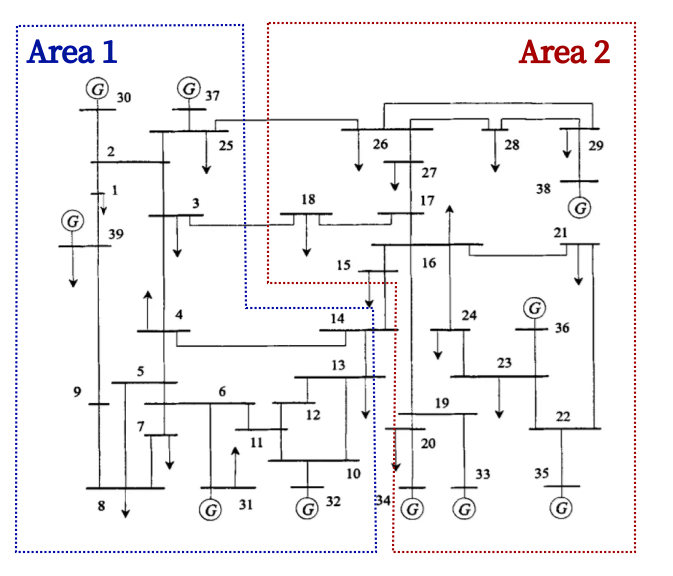
\includegraphics[width=0.8\textwidth]{figures/ieee2areas.png}
    \caption{IEEE39 2 area diagram.}
    \label{fig:ieee39_2areas}
\end{figure}

From the COLMENA side, we deploy multiple agents as docker containers deployed in a single computer. We deploy at two agents per area, where these agents can run both the Distributed MPC role and the roles presented in the previous deliverables (if they respect the requirements). In each area we deploy:

\begin{itemize}
    \item Agent 1: Agent with requirement ('generator', 'solver') 
    \item Agent 2: Agent with requirement ('converter') 
\end{itemize}

On the simulation side, we start the simulation with a grid in steady state conditions. We set up multiple scenarios with the objective of seeing how the different roles act in the grid to counteract this perturbation. We set up the Distributed MPC with a horizon of 3 seconds and a time step of 0.1 seconds.

\subsection{Results}

We define a perturbation at $t=3s$ that consists in a load suddenly doubling. This perturbation provokes a drop in frequency. The Distributed frequency optimizer role activates 10 seconds after the KPI is broken since it needs time to set up. Once the role is activated the frequency is brought back closer to the nominal frequency. The grid does not come back perfectly to the nominal frequency because of the assumptions made in the modelling of the grid. The final oscillations can then be cancelled by the Automatic Response Control.

\begin{figure}[ht]
    \centering
    \begin{minipage}{0.45\textwidth}
        \centering
        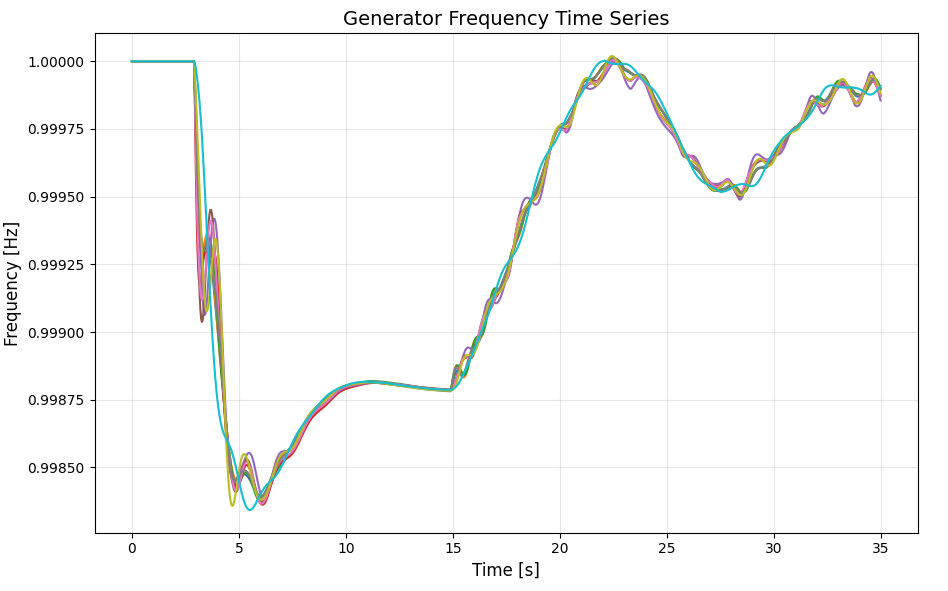
\includegraphics[width=\textwidth]{figures/mpc_load.png}
        \caption{Frequency Time Series - Distributed MPC}
        \label{fig:frequency_response_1}
    \end{minipage}%
    \hspace{0.1cm}  % Adds horizontal space between the figures
    \begin{minipage}{0.45\textwidth}
        \centering
        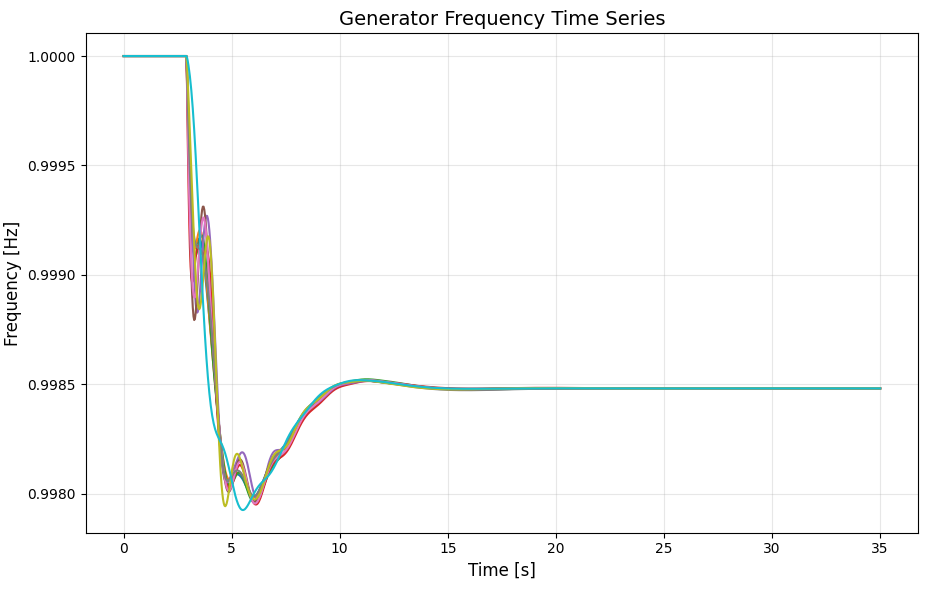
\includegraphics[width=\textwidth]{figures/non_mpc_load.png}
        \caption{Frequency Time Series - Default}
        \label{fig:frequency_response_2}
    \end{minipage}
\end{figure}

Other scenarios available in the prototype's repository are also capable of restoring the grid's frequency. 

\newpage
\section{Milestone Analysis}

\subsection*{Milestone 1}

The final version of the prototype is now fully functional and has been successfully deployed. This version leverages the tools provided by Colmena to enable scalable, modular deployment of decentralized control algorithms. It has been extensively tested using multiple contingency scenarios, including generator outages, line outages and loads increases to validate the robustness of power converter responses under possible stress conditions. The response of the COLMENA control in these scenarios validates the capacity of the roles to respond to perturbations and restore the original frequency. The different testcases along with the prototype are available in the following online repository \cite{repo:colmenaeroots}.

\subsection*{Milestone 2}

The prototype has been successfully deployed on an eRoots machine, following a collaborative effort between eRoots engineers and BSC staff working to overcome possible difficulties during the development. We ensured compatibility with the required software stack and performance expectations. The specific andes app tasked with running the simulation is also available as a docker container in case it is needed further testing is needed. 

\newpage
\section{Future Work}

The results from the simulations validate that deploying frequency control using the COLMENA framework is an effective approach for maintaining grid stability. The system successfully managed frequency deviations, responding to disturbances in a timely manner and restoring the frequency to its nominal value. This demonstrates the robustness and effectiveness of COLMENA's decentralized control strategy, confirming its potential as a reliable solution for frequency regulation in power grids.

The next steps in the development of the COLMENA framework will focus on scaling the system to handle larger and more complex grid structures. This will involve conducting tests in grids with additional areas to assess the scalability of the Distributed MPC controller. Additionally, we will evaluate the framework's performance by validating COLMENA's capabilities in terms of speed and accuracy, ensuring that it can handle the increased computational demands of larger grids while maintaining the desired control precision. These tests will help to refine the system's robustness and efficiency in real-world applications.

\newpage
\nocite{*}  
\printbibliography
\end{document}